% \documentclass[../../Orator]{subfiles}
\documentclass[class={myRUCProject}, crop=false]{standalone}
\IfStandalone{%
    \import{../../}{customCommands}
    \import{../../}{INP-00-glossary}
    }{}
    
\begin{document}

The FitzHugh-Nagumo model can be written in many ways, one of which is as follows.
\begin{sysEquation}
    \ode{V} &= V - \frac{V^{3}}{3} - W + R\,\curr_{\rmm{ext}} \\
    \phi \, \ode{W} &= V + a - b\,W
\end{sysEquation}

\(V\) is the membrane potential, \(W\) is the recovery variable, and \(\curr_{\rmm{ext}}\) is the external current \cite{Sherwood2014}. 
%The original values for the constants are \(a=0.7\), \(b=0.8\), and \(\phi=0.08\) \cite{Sherwood2014}. 
For the sake of analysis, one can just choose to not apply external current, \(\br{\curr_{\rmm{ext}} = 0}\).
For these values, the \glspl{gls:nullcline} look like \Cref{fig:nullclines-original}. 
Nullclines can be identified by solving each term of the system for 0. 
If \(b\) is made to be \(b\leq0\), there will be 3 \gls{gls:equil}. However, as the model is restricted to \(a,b>0\) there is no need to consier such cases. 
\begin{align}
    \ode{V} &= 0 & \ode{W} &= 0\\
    \intertext{the general solutions can be found as:} 
    V &= b\,W - a &  W &= V - \frac{V^3}{3} %+ I 
\end{align}
When \(a,b>0\) The fixed point is found at \(\br{V,\,W} = \br{c^{1/3},\,\rfrac{a}{b}}, c\in\R,\) 
The Jacobian matrix derived from the model; 
\begin{equation}
    J_{\br{V,\,W}} = 
    \begin{bmatrix}
        1 - V^2 & -1 \\
        1 & b
    \end{bmatrix}    
\end{equation}


% \begin{figure}[ht]
%     \centering
%     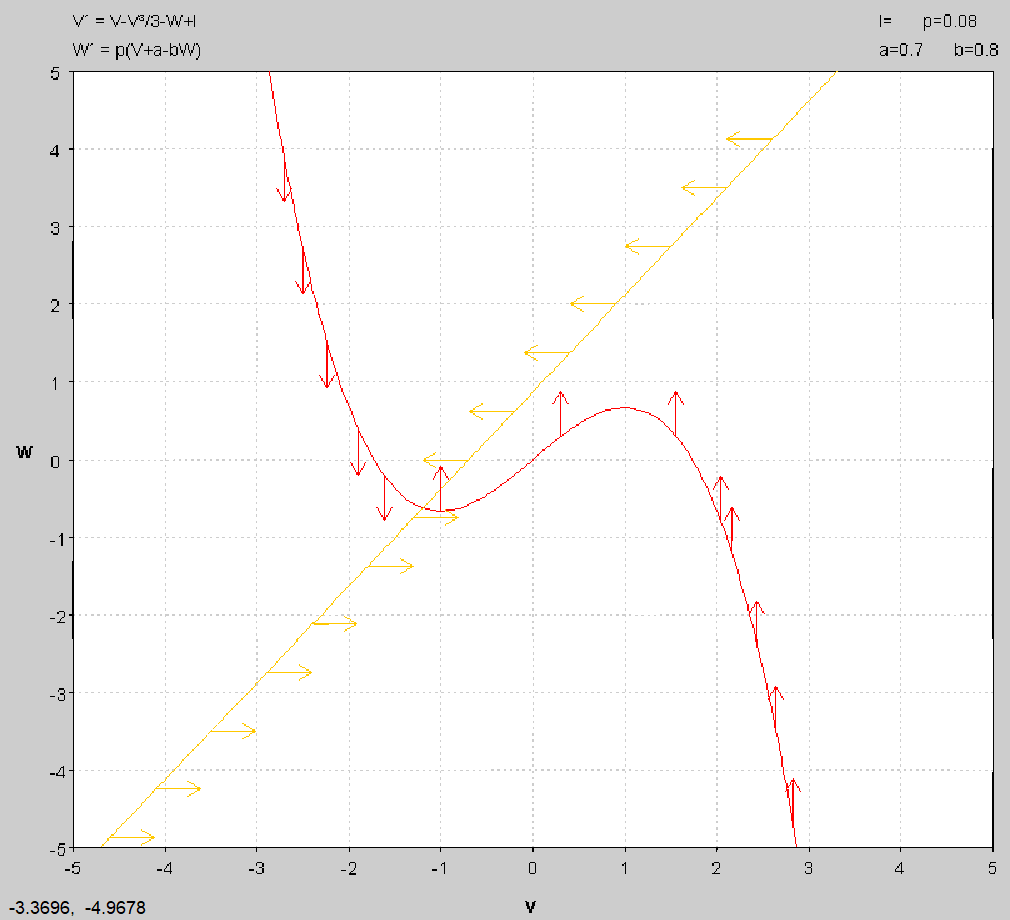
\includegraphics[width=0.7\textwidth]{Pictures/Alex/Nullclines - original.PNG}
%     \caption{\Glspl{gls:nullcline} for \(I=0\), \(a=0.7\), \(b=0.8\), and \(\phi=p=0.08\)}
%     \label{fig:nullclines-original}
% \end{figure}

% As can be seen in \Cref{fig:nullclines-original} there is only one \gls{gls:equil}. 
% This is located at \((-1.1994, -0.62426)\). 
% This is a \gls{gls:spiral}. 




% This can be seen in \Cref{fig:nullclines-negative}.s
% \begin{figure}[ht]
%     \centering
%     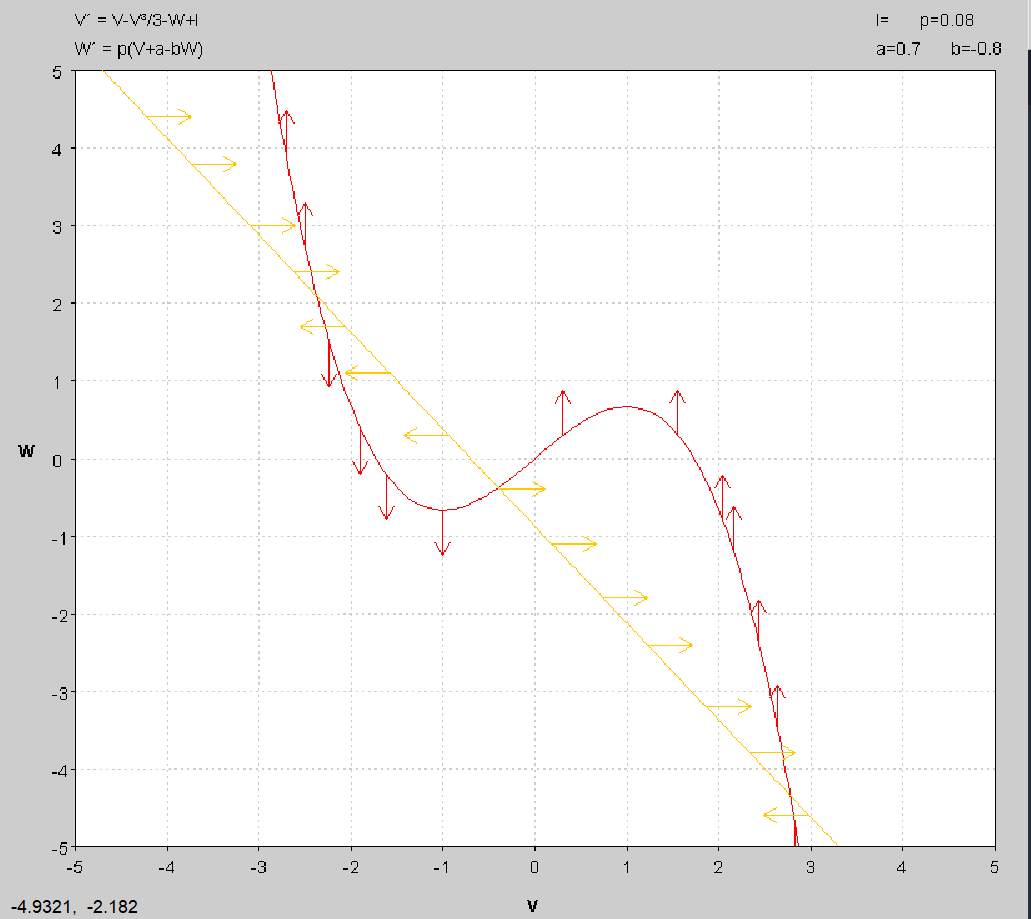
\includegraphics[width=0.7\textwidth]{Pictures/Alex/Nullclines - negative.PNG}
%     \caption{\Glspl{gls:nullcline} for \(I=0\), \(a=0.7\), \(b=-0.8\), and \(\phi=p=0.08\)}
%     \label{fig:nullclines-negative}
% \end{figure}
% Here the \glspl{gls:equil} are at \((-2.376, 2.0949)\), \((-0.39825, -0.37719)\), and \((2.7742, -4.3428)\). The first and last are \glspl{gls:saddle} and the middle is a \gls{gls:nodal}. A saddle point is a point that is a local maximum in one direction and a local minimum in the other direction. Therefore, it is neither a maximum nor a minimum, it is a saddle point. It has eigenvalues satisfying \(\lambda_{1} < 0 < \lambda_{2}\)  A nodal source is a point where the system moves away from the point. It has eigenvalues that satisfy \(\lambda_{1} > \lambda_{2} > 0\).

% HELENA:
% Bifurcation analysis, bifurcation plot

\begin{comment}
    Why do we have 1/3 fixed points?
        Because of the slope of W???
        But why in a biological sense?
\end{comment}

\end{document}